\documentclass{article}
\usepackage{amsmath}
\usepackage{xcolor}
\usepackage{gensymb}
\usepackage{ragged2e}
\usepackage{graphicx}
\usepackage{gensymb}
\usepackage{mathtools}
\newcommand{\mydet}[1]{\ensuremath{\begin{vmatrix}#1\end{vmatrix}}}
\providecommand{\brak}[1]{\ensuremath{\left(#1\right)}}
\providecommand{\norm}[1]{\left\lVert#1\right\rVert}
\newcommand{\solution}{\noindent \textbf{Solution: }}
\newcommand{\myvec}[1]{\ensuremath{\begin{pmatrix}#1\end{pmatrix}}}
\let\vec\mathbf
\begin{document}
\begin{center}
        \textbf\large{CHAPTER-9 \\ AREAS OF PARALLELOGRAMS AND TRIANGLES}
\end{center}
\section{Exercise 9.2}
Q1. In the figure given below, $ABCD$ is a parallelogram, $AE \perp DC$ and $CF \perp AD$.If $AB = 16cm$, $AE = 8cm$ and $CF = 10cm$, find $AD$.\\
\textbf{Construction}\\
\begin{figure}[h]
 \begin{center}
  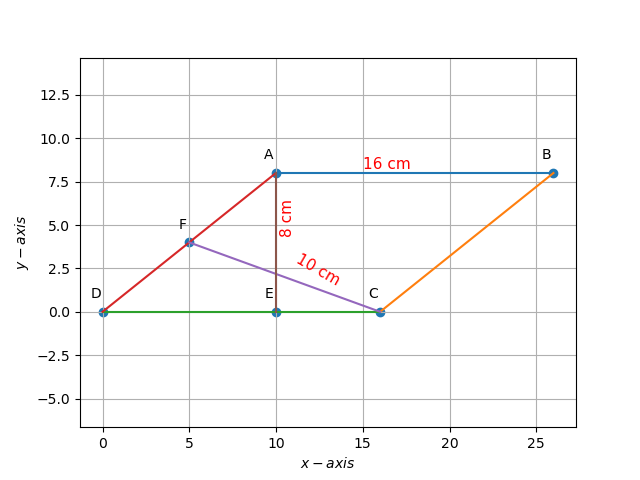
\includegraphics[width=\columnwidth]{fig1.png}
 \end{center}
 \caption{Parallelogram ABCD}
 \label{fig:Fig1}
\end{figure}\\
\pagebreak
The following table displays the given input parameters :\\
\begin{table}[h]
	\centering
	\begin{tabular}{|c|c|c|}
\hline
Symbol & Value & Description\\
\hline
$x$ & 16cm & $\vec{AB}$ \\
\hline
$a$ & 10cm & $\vec{CF}$ \\
\hline
$b$ & 8cm & $\vec{AE}$ \\
\hline
$\angle{CFD}$ & $90\degree$ & $CF \perp AD$ \\
\hline
$\angle{AED}$ & $90\degree$ & $AE \perp CD$ \\
\hline
\end{tabular}

	\caption{Input Parameters}
	\label{tab:table1}
\end{table}\\
The lengths and angles which are to be found out are displayed in the table below along with their symbols :\\
\begin{table}[h]
	\centering
	\begin{tabular}{|p{2cm}|p{2cm}|p{2cm}|}
\hline
\multicolumn{3}{|c|}{Truth table}\\
\hline
R& S& A\\
\hline
0& 0& 0\\
\hline
0& 1& 1\\
\hline
1& 0& 1\\
\hline
1& 1& 0\\
\hline
\end{tabular}

	\caption{Unknown Parameters}
	\label{tab:table2}
\end{table}\\
The input co-ordinates of the above parallelogram is $\vec{D}$ which is at the origin.The rest of the point co-ordinates can be derived based on this assumption in the following way which is shown in the table below :\\
\begin{table}[h]
	\centering
	\begin{tabular}{|c|c|c|}
\hline
Symbol & Description\\
\hline
c & $\norm{\vec{D} -\vec{C}}$ \\
\hline
r & $\norm{\vec{A} -\vec{D}}$ \\
\hline
d & $\norm{\vec{D} - \vec{E}}$\\
\hline
b & $\norm{\vec{A} - \vec{E}}$\\
\hline
$\theta$ & $\angle{\vec{D}}$ \\
\hline
\end{tabular}

	\caption{Unknown Co-ordinates}
	\label{tab:table3}
\end{table}\\
\textbf{Deriving the Unknown lengths and angles in terms of known and derived parameters :}\\
\begin{enumerate}
	\item \textbf{Deriving c:}\\
		From Figure\ref{fig:Fig1}, $c$ is  parallel to $l$(AB paralle to CD).So,
		\begin{align}
			c = l\\
			\label{eq:1}
		\end{align}
	\item \textbf{Deriving d:}\\
		From $\triangle{ADE}$,\\
		\begin{align}
			\cos{\theta} = \frac{DE}{AD} = \frac{d}{r}\\
			\implies d = r\cos{\theta}\\
			\label{eq:2}\\
		\end{align}
	\item \textbf{Deriving r:}\\
		From $\triangle{ADE}$,\\
		\begin{align}
			\sin{\theta} = \frac{AE}{AD} = \frac{b}{r}\\
			\implies r = \frac{b}{\sin{\theta}}\\
			\label{eq:3}\\
		\end{align}
	\item \textbf{Deriving f:}\\
		From $\triangle{DFC}$,\\
		\begin{align}
			\cos{\theta} = \frac{DF}{DC} = \frac{f}{c}\\
			\implies f = c\cos{\theta}\\
			\label{eq:4}\\
		\end{align}
	\item \textbf{Finding $\theta$:}\\
		From $\triangle{DFC}$,\\
		\begin{align}
			\sin{\theta} = \frac{CF}{CD} = \frac{a}{c}\\
			\label{eq:5}\\
			\implies \theta = \sin^{-1}\frac{a}{c}\\
			\label{eq:6}\\
		\end{align}
\end{enumerate}
From \ref{eq:1},\ref{eq:2},\ref{eq:3},\ref{eq:4} and \ref{eq:6}, table\ref{tab:table2} can be modified as :\\
\begin{table}[h]
	\centering
	\begin{tabular}{|c|c|c|}
\hline
Symbol & value & Description\\
\hline
$c$ & $l$ & DC\\
\hline
$r$ & $\frac{b}{\sin{\theta}}$ & AD \\
\hline
$d$ & $r\cos{\theta}$ & DE \\
\hline
$\theta$ & $\sin^{-1}\frac{a}{c}$ & $\angle{D}$ \\
\hline
$f$ & $c\cos{\theta}$ & DF\\
\hline
\end{tabular}


	\caption{Unknown parameters in terms of known and derived parameters}
	\label{tab:table4}
\end{table}\\
\textbf{Deriving co-ordinates in terms of known and derived parameters:}\\
Based on table\ref{tab:table4}, table\ref{tab:table3} can be modified as follows :\\
\begin{table}[h]
	\centering
	\begin{tabular}{|c|c|c|}
\hline
Point & Co-ordinates\\
\hline
$\vec{A}$ & $\myvec{b\cot{\theta}\\b}$\\
\hline
$\vec{B}$ & $\vec{A} + \vec{C}$\\
\hline
$\vec{C}$ & $\myvec{c\\0}$\\
\hline
$\vec{E}$ & $\myvec{r\cos{\theta}\\0}$\\
\hline
$\vec{F}$ & $\frac{k\vec{A} + \vec{D}}{k + 1}$\\
\hline
\end{tabular}

	\caption{Co-ordinates in terms of known and derived co-ordinates}
	\label{tab:table5}
\end{table}\\
\textbf{Finding Co-ordinates:}\\
\begin{enumerate}
	\item \textbf{Co-ordinates of A:}\\
		From \ref{eq:6},the value of $\theta$ is :\\
		\begin{align}
			\theta = \sin^{-1}\frac{a}{c} = \sin^{-1}\frac{10}{16} \\
			\implies \theta = 38.68\degree\\
		\end{align}
		So, co-ordinates of $\vec{A}$ can be derived from table\ref{tab:table5} and they are :\\
		\begin{align}
			\vec{A} = \frac{8}{\sin{38.68}}\myvec{\cos{38.68}\\\sin{38.68}}\\
			\implies \vec{A} = \myvec{10\\8}\\
			\end{align}
	\item \textbf{Co-ordinates of B:}\\
		From table\ref{tab:table5},co-ordinates of $\vec{B}$ are :\\
		\begin{align}
			\vec{B} = \myvec{10\\8} + \myvec{16\\0}\\
			\vec{B} = \myvec{26\\8}\\
		\end{align}
	\item \textbf{Co-ordinates of C are :}\\
		From table\ref{tab:table5},co-ordinates of $\vec{C}$ are :\\
		\begin{align}
			\vec{C} = ce_1 = \myvec{c\\0}\\
			\implies \vec{C} = \myvec{16\\0}\\
		\end{align}
	\item \textbf{Co-ordinates of E :}\\
		From \ref{eq:3}, the value of $r$ is :\\
		\begin{align}
			r = \frac{8}{\sin{38.68}} = 12.8cm\\
			\label{eq:7}
		\end{align}
		From table\ref{tab:table5},co-ordinates of $\vec{E}$ are :\\
		\begin{align}
			\vec{E} = (12.8)\cos{38.68}\myvec{1\\0}\\
			\implies \vec{E} = \myvec{10\\0}\\
		\end{align}
	\item \textbf{co-ordinates of F:}\\
		From table\ref{tab:table5},co-ordinates of $\vec{F}$ are :\\
		\begin{align}
			\vec{F} = (16)\cos{38.68}\myvec{\cos{38.68}\\\sin{38.68}}\\
			\implies \vec{F} = \myvec{9.75\\7.8}\\
		\end{align}
\end{enumerate}
So, the final co-ordinates of the  parallelogram are displayed in the table below:\\
\begin{table}[h]
	\centering
	\begin{tabular}{|c|c|}
\hline
Point & Co-ordinates\\
\hline
$\vec{A}$ & $\myvec{10\\8}$\\
\hline
$\vec{B}$ & $\myvec{26\\8}$\\
\hline
$\vec{C}$ & $\myvec{16\\0}$\\
\hline
$\vec{D}$ & $\myvec{0\\0}$\\
\hline
$\vec{E}$ & $\myvec{10\\0}$\\
\hline
$\vec{F}$ & $\myvec{9.75\\7.8}$\\
\hline
\end{tabular}

	\caption{Final Co-ordinates}
	\label{tab:table7}
\end{table}\\
From \ref{eq:7}, we got the length of AD = r = 12.8cm.
\end{document}
